% 
% Annual CCN conference
% Sample LaTeX Two-Page Summary -- Proceedings Format
% based on the prior cognitive science style file

% Original : Ashwin Ram (ashwin@cc.gatech.edu)       04/01/1994
% Modified : Johanna Moore (jmoore@cs.pitt.edu)      03/17/1995
% Modified : David Noelle (noelle@ucsd.edu)          03/15/1996
% Modified : Pat Langley (langley@cs.stanford.edu)   01/26/1997
% Latex2e corrections by Ramin Charles Nakisa        01/28/1997 
% Modified : Tina Eliassi-Rad (eliassi@cs.wisc.edu)  01/31/1998
% Modified : Trisha Yannuzzi (trisha@ircs.upenn.edu) 12/28/1999 (in process)
% Modified : Mary Ellen Foster (M.E.Foster@ed.ac.uk) 12/11/2000
% Modified : Ken Forbus                              01/23/2004
% Modified : Eli M. Silk (esilk@pitt.edu)            05/24/2005
% Modified : Niels Taatgen (taatgen@cmu.edu)        10/24/2006
% Modified : David Noelle (dnoelle@ucmerced.edu)     11/19/2014
% Modified : Konrad Kording (koerding@gmail.com) 2/15/2017

\documentclass[10pt,letterpaper]{article}

\usepackage{ccn}
\usepackage{pslatex}
\usepackage{apacite}
\usepackage{graphicx}

\title{Familiarity strengthens visual object representations}
 
\author{{\large \bf Jasper J.F. van den Bosch (vandejjf@bham.ac.uk)} \\
  A Department, 1234 Example Street\\
A City, State 12345 A country
  \AND {\large \bf Cyril Pernet (cyril.pernet@ed.ac.uk)} \\
  A Department, 1234 Example Street\\
A City, State 12345 A country
  \AND {\large \bf Ian Charest (charesti@bham.ac.uk)} \\
  A Department, 1234 Example Street\\
A City, State 12345 A country}


\begin{document}

\maketitle


\section{Abstract}
{
\bf
We are exposed to personally meaningful objects throughout the 
course of our life, and this must  be reflected in the brain. 
Despite evidence for larger brain activity, the impact of 
familiarity on the spatio-temporal dynamics of object recognition 
remains poorly understood. Here we set out to track neural 
representations of familiar and unfamiliar objects in the human 
brain as they evolve in space and time. Participants (n=20), 
saw personally-meaningful and unfamiliar objects matched in 
category and concept (72 images, including faces, bodies, 
places, objects and pets) while we recorded electroencephalography 
(EEG) and functional Magnetic Resonance Imaging (fMRI) (in separate 
sessions). Using similarity-based fusion, we combined the precise 
temporal resolution of EEG with the precise spatial resolution of 
fMRI to map the spatio-temporal trajectories of personally-meaningful 
and unfamiliar object representations. These followed the typical 
cascade of visual processes bilaterally from primary visual cortex 
(V1; ~90ms) through to the ventral and dorsal streams (~130ms). 
Critically, our results strengthen our understanding of the interactions 
between the visual sensory system, the medial temporal lobes, and 
the prefrontal cortex in recognising visual objects. 
}
\begin{quote}
\small
\textbf{Keywords:} 
familiarity; fmri; eeg; rsa
\end{quote}

\section{Introduction}

The things we see everyday vary greatly in how well we know them. 
Many lab experiments on object vision use images of things that 
the participant has not seen before. However, familiarity with 
an object has been observed to improve recognition performance, 
suggesting that it plays a key role in how we process the stimulus. 
This effect has been widely studied in faces; documenting a response 
80ms faster for familiar faces on several tasks (Ramon and Gobbini 2018, 
Visconti di Oleggio Castello et al. 2017). 
Electroencephalography (EEG) studies revealed  amplified neural 
activity in response to familiar objects (Herzmann et al. 2004). 
Functional differences between familiar and unfamiliar objects 
have also been revealed using functional Magnetic Resonance Imaging (fMRI)
\cite{Barense2011-bl,McLelland2014-es,Taylor2009-hw,Trinkler2009-dm} 
Studies increasingly turn to multivariate pattern analyses (MVPA) 
to characterise finer distinctions between experimental conditions 
from the experimental data. For example, Representational Similarity 
Analyses (RSA; Kriegeskorte et al. 2008), enables measuring fine-grained 
representational geometries in different regions of the brain, 
and testing specific hypothesis with computational or theoretical 
models (Kriegeskorte and Kievit 2013). This yielded an understanding 
of the functional properties of human inferior temporal cortex, 
with activity patterns clustering according to categories 
(Haxby et al. 2001; Kriegeskorte et al. 2008), which in turn are 
reflected in perceived similarity judgements (Mur et al. 2013).  
Linear classifiers applied to M/EEG data further revealed that 
individual object exemplars can be decoded from around 100ms 
after their presentation (Carlson et al. 2013). 

Representational geometries measured using RSA can be 
compared between measurement modalities, lending it to 
map object representations in space and time 
(Cichy et al. 2014; Cichy et al. 2016). One key aspect of 
familiarity is its idiosyncratic nature; we each have a 
different level of familiarity with a given thing. In previous work 
(Charest et al. 2014), we observed that the object representations 
in IT reflect such differences, and that these are stable across days. 
More recently, a study of face perception using RSA found that 
representations of famous celebrity faces, which have a degree of 
familiarity for all participants, are enhanced early on when 
compared to unfamiliar faces (Dobs et al. 2019). 

Here, we collected EEG and fMRI data while participants viewed 
personally meaningful or unfamiliar images, from a wide range 
of object categories including animals, bodies, faces, objects, 
and places. Using RSA, we combine data from both modalities to 
reveal the role of familiarity in object as representations 
unfold in space and time.

\begin{figure}[t]
\begin{center}
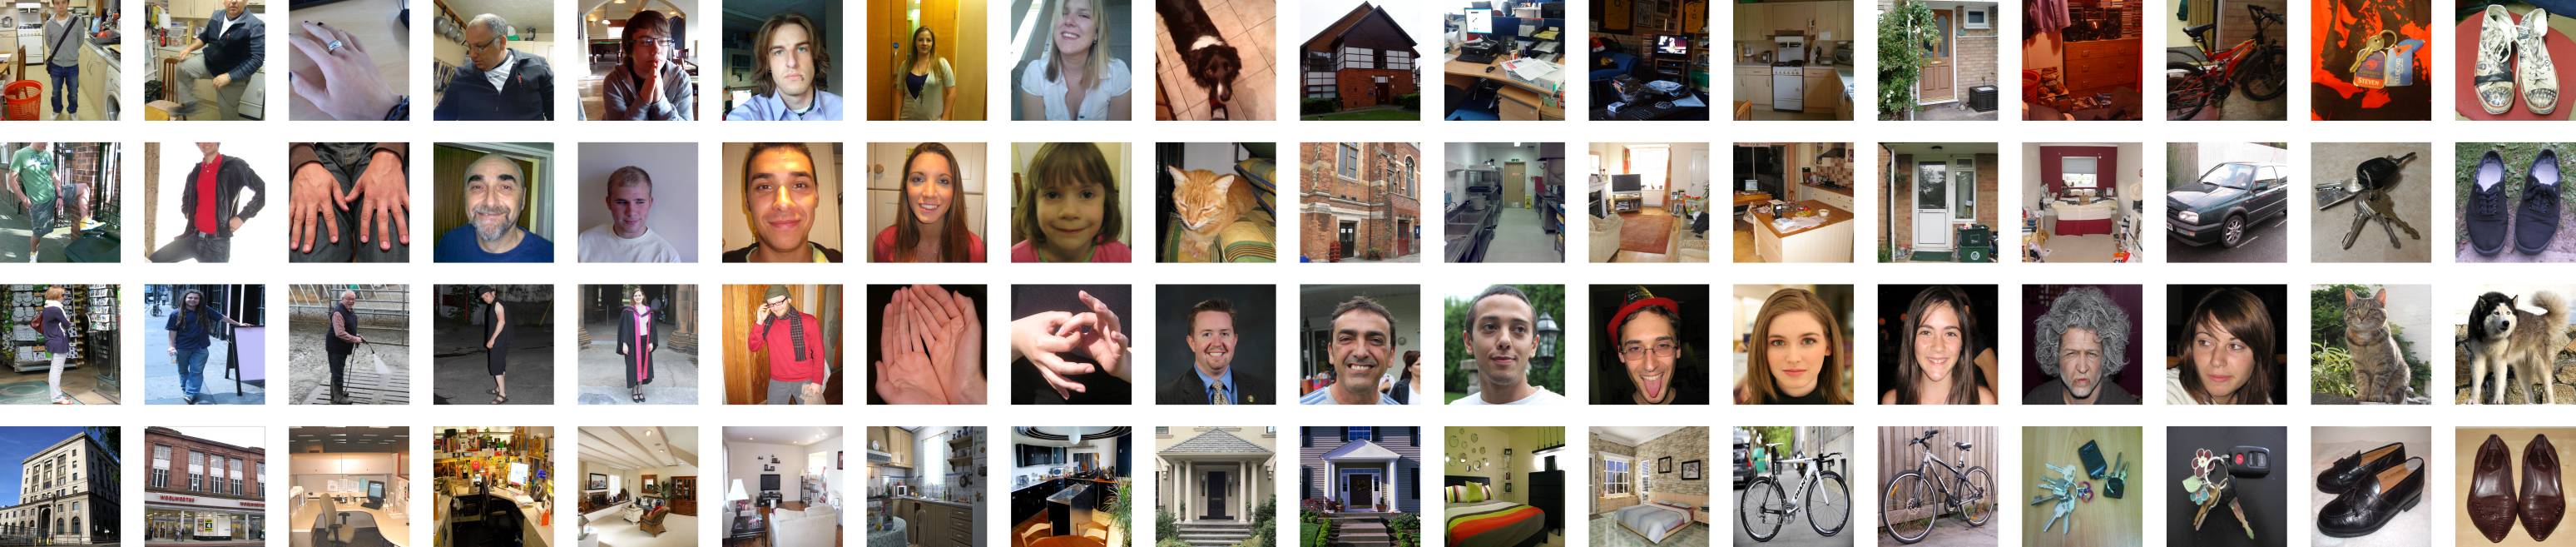
\includegraphics[width=\linewidth]{figures/figure1.png}
\end{center}
\caption{
  Stimulus materials. The first two rows depict example 
  stimuli for a pair of participant. The bottom row depicts the 
  visual object images shown to all pairs of participants.
} 
\label{sample-figure}
\end{figure}

\section{First Level Headings}

First level headings should be in 12~point, initial caps, bold and
centered. Leave one line space above the heading and 1/4~line space
below the heading.


\subsection{Second Level Headings}

Second level headings should be 11~point, initial caps, bold, and
flush left. Leave one line space above the heading and 1/4~line
space below the heading.


\subsubsection{Third Level Headings}

Third level headings should be 10~point, initial caps, bold, and flush
left. Leave one line space above the heading, but no space after.




\subsection{Footnotes}

Indicate footnotes with a number\footnote{Sample of the first
footnote.} in the text. Place the footnotes in 9~point type at the
bottom of the column on which they appear. Precede the footnote block
with a horizontal rule.\footnote{Sample of the second footnote.}


\subsection{Tables}

Number tables consecutively. Place the table number and title (in
10~point) above the table with one line space above the caption and
one line space below it, as in Table~\ref{sample-table}. You may float
tables to the top or bottom of a column, or set wide tables across
both columns.

\begin{table}[!ht]
\begin{center} 
\caption{Sample table title.} 
\label{sample-table} 
\vskip 0.12in
\begin{tabular}{ll} 
\hline
Error type    &  Example \\
\hline
Take smaller        &   63 - 44 = 21 \\
Always borrow~~~~   &   96 - 42 = 34 \\
0 - N = N           &   70 - 47 = 37 \\
0 - N = 0           &   70 - 47 = 30 \\
\hline
\end{tabular} 
\end{center} 
\end{table}


\subsection{Figures}

Make sure that the artwork can be printed well (e.g. dark colors) and that 
the figures make understanding the paper easy.
 Number figures sequentially, placing the figure
number and caption, in 10~point, after the figure with one line space
above the caption and one line space below it, as in
Figure~\ref{sample-figure}. If necessary, leave extra white space at
the bottom of the page to avoid splitting the figure and figure
caption. You may float figures to the top or bottom of a column, or
set wide figures across both columns.

\begin{figure}[ht]
\begin{center}
\fbox{CCN figure}
\end{center}
\caption{This is a figure.} 
\label{sample-figure}
\end{figure}


\section{Acknowledgments}

Place acknowledgments (including funding information) in a section at
the end of the paper.


\section{References Instructions}

Follow the APA Publication Manual for citation format, both within the
text and in the reference list, with the following exceptions: (a) do
not cite the page numbers of any book, including chapters in edited
volumes; (b) use the same format for unpublished references as for
published ones. Alphabetize references by the surnames of the authors,
with single author entries preceding multiple author entries. Order
references by the same authors by the year of publication, with the
earliest first.

Use a first level section heading, ``{\bf References}'', as shown
below. Use a hanging indent style, with the first line of the
reference flush against the left margin and subsequent lines indented
by 1/8~inch. Below are example references for a conference paper, book
chapter, journal article, dissertation, book, technical report, and
edited volume, respectively.

\nocite{ChalnickBillman1988a}
\nocite{Feigenbaum1963a}
\nocite{Hill1983a}
\nocite{OhlssonLangley1985a}
% \nocite{Lewis1978a}
\nocite{Matlock2001}
\nocite{NewellSimon1972a}
\nocite{ShragerLangley1990a}


\bibliographystyle{apacite}

\setlength{\bibleftmargin}{.125in}
\setlength{\bibindent}{-\bibleftmargin}

\bibliography{vandenbosch}


\end{document}
